\documentclass[../../relatorio.tex]{subfiles}

\begin{document}

\subsection{Bolsa de Valores de São Paulo (BOVESPA)}

\begin{figure}[!ht]
  \begin{minipage}{0.70\textheight}
    \centering
      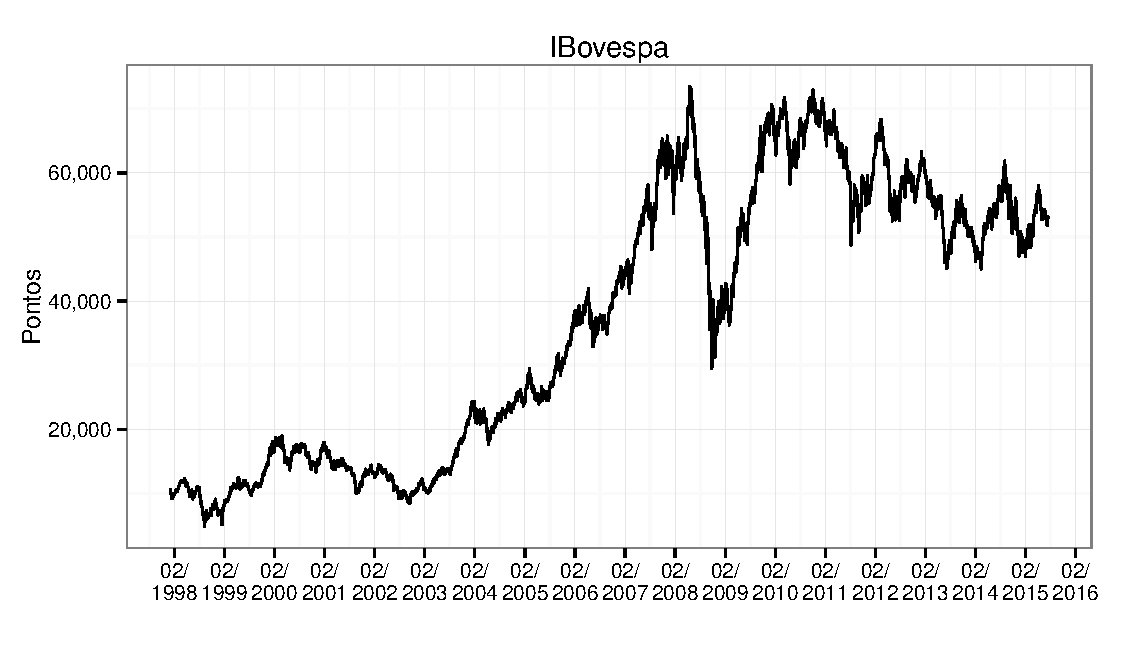
\includegraphics[width=17cm]{Bovespa.pdf}
  \end{minipage}
\end{figure}

\textbf{Índice Bovespa (Ibovespa)} é o mais importante indicador do desempenho médio das cotações das ações negociadas na Bolsa de Valores de São Paulo. É formado pelas ações com maior volume negociado nos últimos meses. O valor atual representa a quantia, em moeda corrente, de uma carteira teórica de ações, constituída em 2 de janeiro de 1968, a partir de uma aplicação hipotética. Atribuiu-se o valor-base de 100 a um lote-padrão cujo carteira se avoluma sem receber mais nenhum aporte, com o acréscimo exclusivo de proventos gerados pelas ações que compõem o lote-padrão tais como a reinversão de dividendos, exercício de direitos e recebimento de bonificações.

Para que sua representatividade se mantenha ao longo do tempo, a composição da carteira teórica é reavaliada a cada quatro meses. Essa reavaliação é feita com base nos últimos 12 meses onde são verificadas alterações na participação de cada ação.

O índice é calculado em tempo real, considerando instantaneamente os preços de todos os negócios efetuados no mercado à vista com ações componentes de sua carteira (lote padrão) e é divulgado pela Bovespa, podendo ser acompanhado on line. \footnote{http://pt.wikipedia.org/wiki/Ibovespa}

\pagebreak


\begin{figure}[!ht]
  \begin{minipage}{\textwidth}
    \centering
      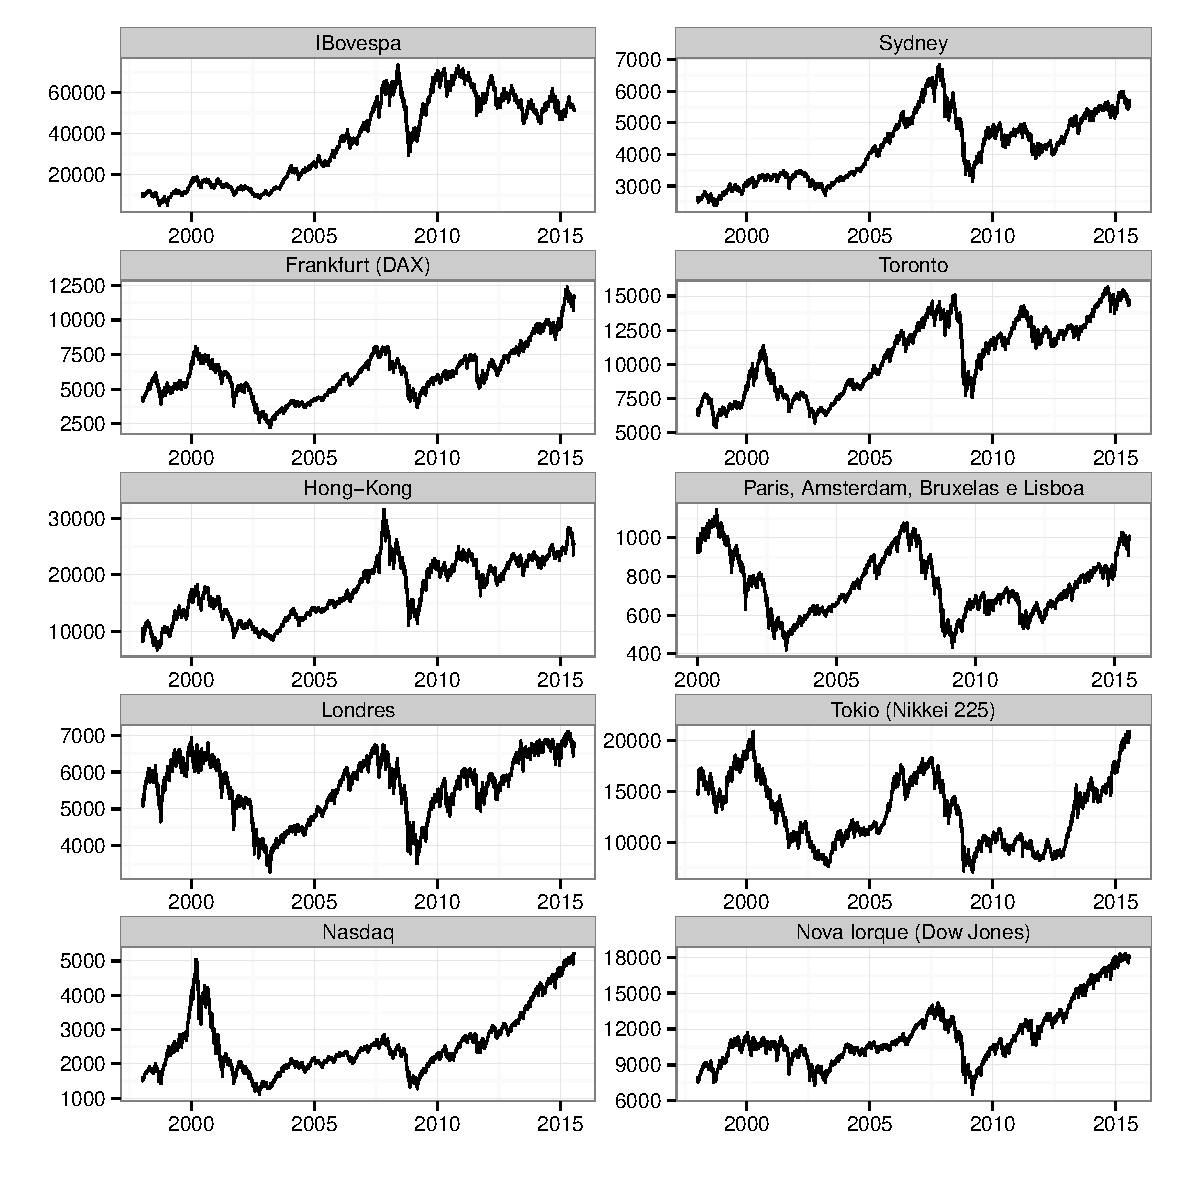
\includegraphics[height=0.9\textheight,width=\textwidth]{BolsasMundo.pdf}
  \end{minipage}
\end{figure}

\pagebreak
\end{document}
